\documentclass[11pt]{article}

\usepackage[T1]{fontenc}
\usepackage[margin=2.5cm]{geometry}
\usepackage{amsmath,amssymb,amsthm}
\usepackage{booktabs,array}
\usepackage{graphicx}
\usepackage{hyperref}

\title{A failure gallery for univariateML: ten maximum-likelihood pathologies}
\author{}
\date{\today}

\newcommand{\E}{\mathbb{E}}
\newcommand{\tr}{\operatorname{tr}}
\newcommand{\Var}{\operatorname{Var}}
\newcommand{\Cov}{\operatorname{Cov}}
\newcommand{\argmin}{\operatorname*{arg\,min}}
\newcommand{\argmax}{\operatorname*{arg\,max}}
\newcommand{\cF}{\mathcal{F}}
\newcommand{\code}[1]{\texttt{#1}}

\theoremstyle{plain}
\newtheorem{theorem}{Theorem}
\newtheorem{lemma}{Lemma}
\newtheorem{corollary}{Corollary}
\newtheorem{proposition}{Proposition}
\theoremstyle{definition}
\newtheorem{definition}{Definition}
\theoremstyle{remark}
\newtheorem*{remark}{Remark}

\begin{document}
\maketitle

\section*{Purpose}

Ten classical maximum-likelihood failure phenomena, each with a minimal
reproducer against the current \code{univariateML} fitters and a
profile-likelihood figure. Companion to \code{notes/ml-behaviour.tex}
(Hellinger closure and escape taxonomy for all 100 families); this note
picks out named textbook pathologies rather than surveying every family.
Scripts: \code{notes/failure-gallery/fig*.R}, run from the repository root
against the package built by \code{just test}. Source material:
\code{roadmap/2026-10-29-classical-failure-families.md},
\code{STATUS.md} (``Write-up''), and the \code{notes/evaluations/2026-10-29-*}
job reports cited in each section.

\section{Two-adjacent-integer escape of the discretized normal and gamma}
\label{sec:dnormgamma}

\code{dnorm} and \code{dgamma} record the integer part of a latent
continuous normal or gamma variable: $P(X=k)=F(k+1)-F(k)$. With both
parameters free, the MLE exists and is unique whenever the sample range is
at least two (strict concavity in $(\mu/\sigma,1/\sigma)$ for the normal,
Burridge 1981 \cite{burridge1981}; an analogous argument for the gamma). On
exactly \emph{two adjacent integers} $k,k+1$ with lower-cell fraction $p$,
every finite fit is strictly dominated by the saturated two-point law: no
MLE exists, and the supremum is approached along $\mu=k+1-\sigma\Phi^{-1}(p)$,
$\sigma\downarrow0$ (or the matching gamma path), where the two cell
probabilities tend to $p$ and $1-p$.

Minimal reproducer (seven observations at 3, three at 4):
\begin{verbatim}
> mldnorm(c(rep(3, 7), rep(4, 3)))
Error: The maximum likelihood estimator does not exist on two adjacent
integers; use `mlbinom(x - k, size = 1)` with k = min(x).
\end{verbatim}
The saturated bound is $7\log(0.7)+3\log(0.3)=-6.108643020549$, attained
only in the limit (Figure~\ref{fig:dnormgamma}).

This is not a small-sample artefact: in $10^4$ replicates per cell (seed
20261029), \code{floor(rnorm(n, 4, .2))} lands on two adjacent integers in
100\%, 99.99\% and 99.90\% of samples at $n=20,100,1000$, and
\code{round(rnorm(n, 3.5, .2))} in 100\%, 99.99\% and 99.95\%
(\code{notes/evaluations/2026-10-29-dnormgamma-escape-frequency.csv}); the
escape probability depends on how tightly the latent spread is resolved by
integer binning, not on $n$, and need not vanish as $n\to\infty$. The
discretized gamma has the same two-point face and the same non-vanishing
escape rate at a narrow shape (\code{dgamma\_concentrated} in the same
table).

\begin{figure}[h]
\centering
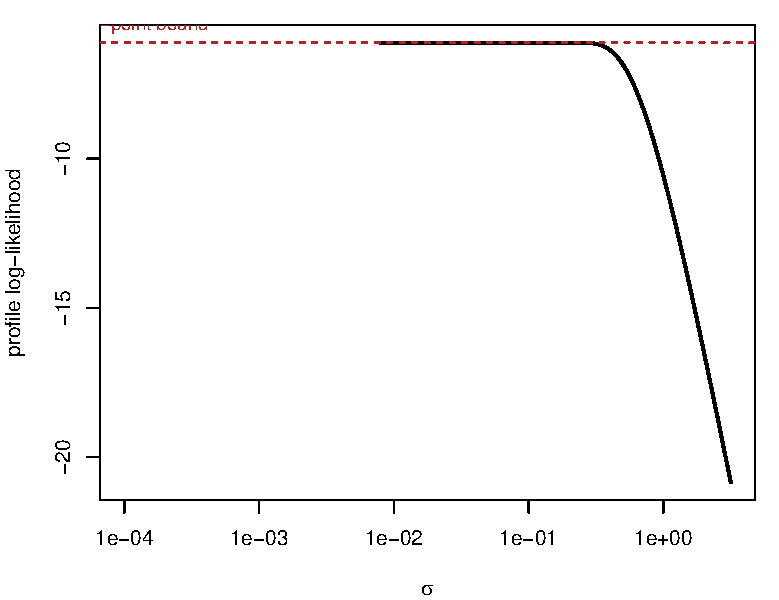
\includegraphics[width=0.62\textwidth]{failure-gallery/fig01-dnormgamma.pdf}
\caption{Profile log-likelihood of the discretized normal (location
re-optimized at each $\sigma$) on seven 3s and three 4s, against the
saturated two-point bound.}
\label{fig:dnormgamma}
\end{figure}

\section{Bhattacharjee's normal face}
\label{sec:bhatt}

The Bhattacharjee law is a normal--uniform convolution with scales
$(\sigma,a)$, $a\ge0$; $a=0$ is exactly the normal. Unlike the escapes
below, $a\ge0$ is a genuine boundary of the parameter space, not a point
outside it (decision A2, \code{notes/evaluations/2026-10-29-p0-summary.md}):
the one-sided score of the profile likelihood at $a=0^+$ has the sign of
$3-K$, $K$ the sample kurtosis, so $a=0$ is attained whenever $K>3$ and an
interior $a>0$ improves the fit whenever $K<3$. Because sample kurtosis
fluctuates around 3 with a non-vanishing spread at every $n$, this is a
boundary phenomenon that does not disappear as $n\to\infty$, unlike the
exponential and Poisson escapes of Sections~\ref{sec:dnormgamma} and
\ref{sec:exppois}.

\begin{verbatim}
> x <- rnorm(80)   # seed 1; sample kurtosis 3.26 > 3
> mlbhatt(x)
Maximum likelihood estimates for the Bhattacharjee model
    mu   sigma       a
0.1061  0.8952  0.0000
\end{verbatim}
$a=0$ is returned exactly (the boundary MLE, not an error), with
logLik $=-104.6556$; the profile is strictly decreasing in $a$ away from
zero (Figure~\ref{fig:bhatt}). A seeded study of 100 normal samples per
size (\code{notes/evaluations/2026-10-29-slashbhatt-report.md}) finds the
normal face selected in 21/100, 40/100 and 46/100 replicates at
$n=20,100,1000$; the complementary mass splits between the uniform face
(common at $n=20$, rare at $n\ge100$) and interior fits.

\begin{figure}[h]
\centering
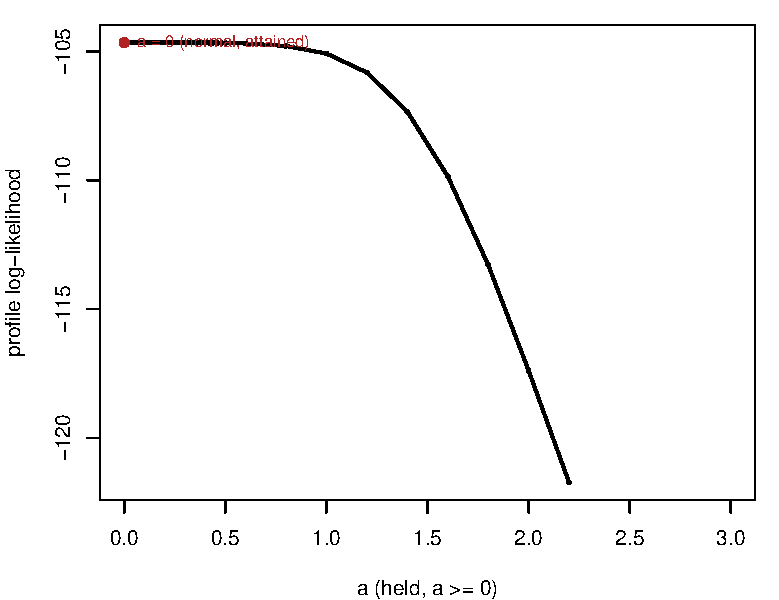
\includegraphics[width=0.62\textwidth]{failure-gallery/fig02-bhatt.pdf}
\caption{Profile log-likelihood of the Bhattacharjee model over the held
half-width $a\ge0$, normal sample ($K=3.26$), attained maximum at $a=0$.}
\label{fig:bhatt}
\end{figure}

\section{Generalized beta: power samples escaping to a shorter power law}
\label{sec:genbeta}

The generalized beta of the first kind, $Y=-\log(X/\theta)\sim$ a
transformed beta, has three shapes $(\alpha,\beta,\tau)$ and a held upper
endpoint $\theta$ (Kleiber and Kotz 2003 \cite{kk2003}). Along
$\alpha\to0$, $\tau\to\infty$ with $\alpha\tau\to\lambda$ fixed and
$\log\beta/\tau\to c\ge0$, $Y\to c+\mathrm{Exp}(\lambda)$: a power law on
$(0,\theta e^{-c})$, an endpoint strictly \emph{shorter} than $\theta$
whenever $c>0$. This happens whenever the data cluster well inside
$(0,\theta)$ rather than filling it, since $\beta\to\infty$ is the only way
the three-shape family can mimic a support shorter than the one it is
held to.

Minimal reproducer ($X=e^{-Y}$, $Y\sim\mathrm{Gamma}(2,\mathrm{rate}=3)$,
not itself a genbeta member):
\begin{verbatim}
> set.seed(2); x <- exp(-rgamma(40, shape = 2, rate = 3))
> mlgenbeta(x, scale = 1)
Error: Generalized beta selects a limiting power law. Use `mlpower`.
> mlpower(x)
alpha (endpoint) = 0.8778, beta (shape) = 1.8975, logLik = 11.9165
\end{verbatim}
\code{max(x)} $=0.8778$ against the held \code{scale = 1}: the escaping
model's endpoint is the sample maximum, well short of the scale the fit
was constrained to. In a seeded catalogue of this generator
(\code{notes/evaluations/2026-10-29-genbeta-report.md}), 20 replicates at
$n=50$ split 4 interior, 5 power (this escape), 11 unit-gamma (the other
nondegenerate limit, $\alpha\to\infty,\tau\to0,\alpha\tau$ fixed).

\begin{figure}[h]
\centering
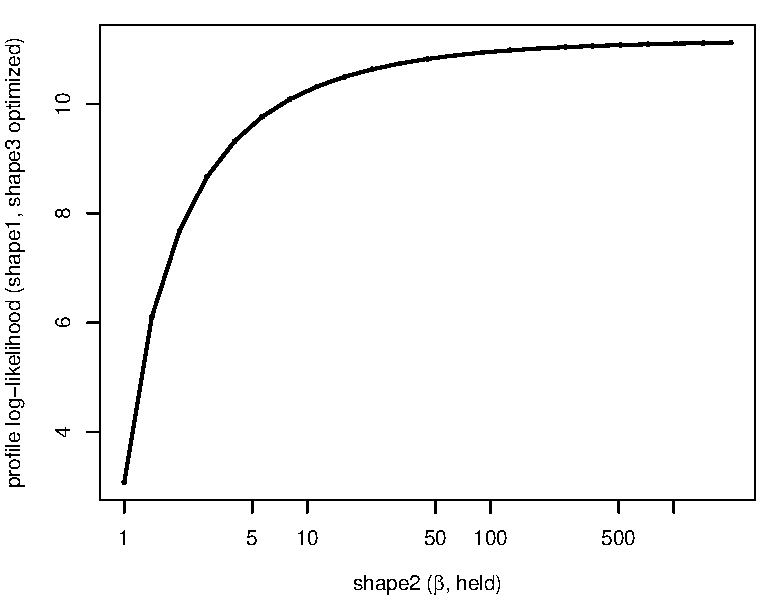
\includegraphics[width=0.62\textwidth]{failure-gallery/fig03-genbeta.pdf}
\caption{Profile log-likelihood of the generalized beta over the held
shape $\beta$ (the other two shapes optimized), against the power-law
limit with endpoint $\max(x)<\mathrm{scale}$.}
\label{fig:genbeta}
\end{figure}

\section{Tukey lambda: unbounded likelihood as the shape grows}
\label{sec:tlambda}

The Tukey lambda quantile function is $Q(u)=\mu+\sigma(u^\lambda-(1-u)^\lambda)/\lambda$
(Joiner and Rosenblatt 1971 \cite{joiner1971}). With location and scale
free, the likelihood is unbounded as $\lambda\to\infty$: put $\mu$ at an
observation with multiplicity $k\ge1$ and $\sigma=\lambda A$, $A$ exceeding
every other distance to it. Then
\[
  \ell(\lambda) = k\lambda\log2 - n\log\lambda + O(1), \qquad \lambda\to\infty,
\]
so $\ell\to\infty$; no unrestricted MLE exists for any sample. The package
fits only the principal unimodal branch $\lambda\in[-1,1]$ (excluding the
non-upper-semicontinuous U-shaped branch $(1,2)$), with the uniform
($\lambda=1$ or $2$) an attained member rather than an escape.

\begin{verbatim}
> x <- c(-2, -1, 0, 0.3, 1, 3)
> mltlambda(x)
Warning: mltlambda reached a fitting restriction: `lambda` = 1 (upper
bound): lambda <= 1 selects the principal branch; no exemption is proved.
    mu  sigma  lambda
   0.5    2.5    1.0
\end{verbatim}
Direct evaluation of $\ell(\lambda)$ along the escaping path (location at
$x_1=-2$, $\sigma=4\lambda$) gives $-12.4766$, $2.07364$, $25.7199$ at
$\lambda=2,40,80$, matching the asymptotic formula and the restricted
fit's value exactly
(\code{notes/evaluations/2026-10-29-tlambda-report.md}); the unrestricted
likelihood overtakes the restricted optimum near $\lambda\approx7$ and
diverges beyond it (Figure~\ref{fig:tlambda}).

\begin{figure}[h]
\centering
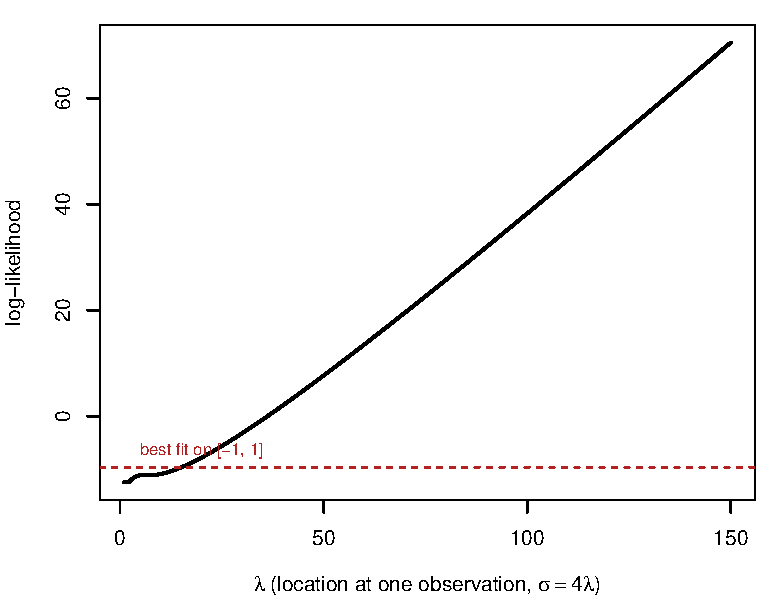
\includegraphics[width=0.62\textwidth]{failure-gallery/fig04-tlambda.pdf}
\caption{Log-likelihood along the diverging path $\mu=x_1$, $\sigma=4\lambda$,
against the best fit on the restricted branch $\lambda\in[-1,1]$.}
\label{fig:tlambda}
\end{figure}

\section{Slash: the exactly-half-tied case}
\label{sec:slash}

The slash density is $f(z)=c(1-e^{-z^2/2})/z^2$, $c=1/\sqrt{2\pi}$,
continuously extended to $c/2$ at $z=0$. At a location $v$ with tie
multiplicity $k$, free-scale collapse ($\sigma\to0$) has likelihood
proportional to $\sigma^{n-2k}$: unbounded for $k>n/2$, zero in the limit
for $k<n/2$, and a finite nonzero constant
$B_v=c^n2^{-n/2}\prod_{x\ne v}|x-v|^{-2}$ exactly at $k=n/2$. At that knife
edge, whether $B_v$ is the global supremum is a variational comparison
with every interior candidate, not a multiplicity count.

Minimal reproducer ($n=20$, ten tied at 0, one at $-1$, nine at 9; exact
rational verification in
\code{cppunivariate/.../distributions/slash/existence-proof.py}):
\begin{verbatim}
> x <- c(rep(0, 10), -1, rep(9, 9))
> mlslash(x)
   mu  sigma
3.554  2.798
\end{verbatim}
$\log B_0=-64.860285$ and $L(\mu=4,\sigma=3)/B_0=1.45605$: an interior
point beats the collapse bound, and the fitter's own global search finds
the interior maximum near $(3.55,2.80)$ rather than the tie at $v=0$
(Figure~\ref{fig:slash}).

\begin{figure}[h]
\centering
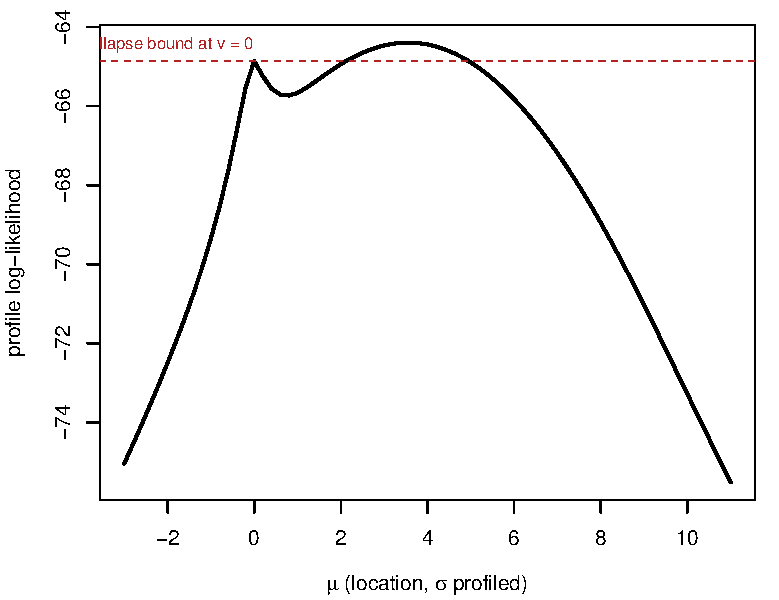
\includegraphics[width=0.62\textwidth]{failure-gallery/fig05-slash.pdf}
\caption{Profile log-likelihood over location (scale profiled), against
the exactly-half-tied collapse bound $B_0$ at $v=0$.}
\label{fig:slash}
\end{figure}

\section{Bimodal half-t degrees-of-freedom profile}
\label{sec:ht}

The half-t density is $f(x;\nu,\sigma)=(2/\sigma)t_\nu(x/\sigma)$, $x\ge0$.
With scale profiled out exactly (its score is monotone in $\sigma$ at
fixed $\nu$), the remaining one-dimensional profile over $\nu$ need not be
unimodal.

\begin{verbatim}
> x <- c(.12773, 12.5979, 3.91782, 2.58658, .138212)
> mlht(x)
    nu  sigma
0.4151 0.3377
\end{verbatim}
This sample has two local maxima of the $\nu$-profile, at
$\nu=0.41508$ (logLik $-11.72979$, the global maximum returned by
\code{mlht}) and $\nu=1.17074$ (logLik $-11.98253$); the half-normal face
($\nu\to\infty$) is lower still, at logLik $-12.59859$
(\code{cppunivariate/.../distributions/ht/README.md}; verified
independently against \code{stats::dt} in Figure~\ref{fig:ht}). A
1200-sample scan over varied sizes and spreads found 32 of 1200 profiles
multimodal (\code{notes/evaluations/2026-10-29-halfdists-report.md}); the
fitter's log-$\nu$ grid plus refinement is not a certified global search.

\begin{figure}[h]
\centering
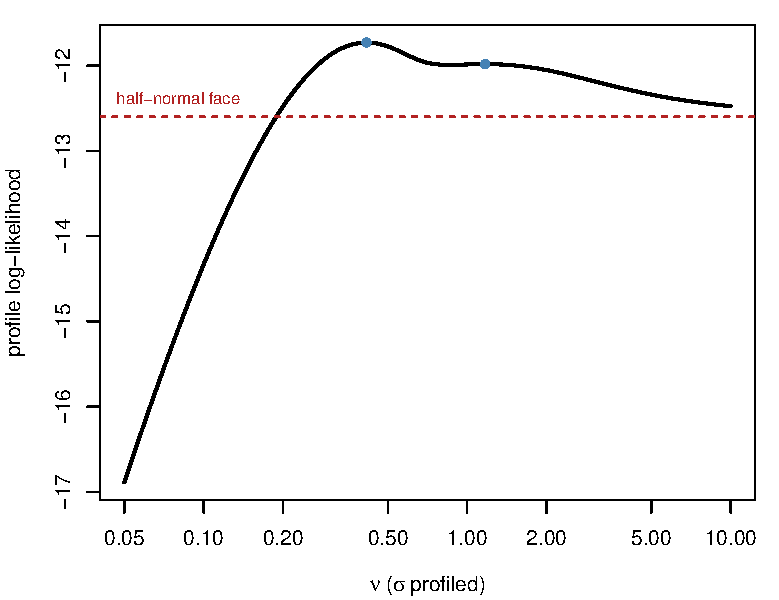
\includegraphics[width=0.62\textwidth]{failure-gallery/fig06-ht.pdf}
\caption{Profile log-likelihood of the half-t over $\nu$ (scale profiled
in closed form), two local maxima marked, against the half-normal face.}
\label{fig:ht}
\end{figure}

\section{Skew-normal: infinite shape and the stationary point at shape zero}
\label{sec:sn}

Azzalini's skew-normal (Azzalini 1985 \cite{azzalini1985}) has direct
parameters $(\xi,\omega,\alpha)$. Two distinct pathologies coexist. First,
$\alpha=0$ is always a stationary point of the profile likelihood: with
$\eta=1/\omega$, $z_i=\eta x_i-h$ standardized at the normal MLE, the
shape score there is $\sqrt{2/\pi}\sum_iz_i=0$ identically (envelope
theorem), and the direct-parameter Fisher information is singular at
symmetry (Azzalini and Capitanio 1999 \cite{azzalinicapitanio1999}; the
remedy is centred mean/sd/skewness coordinates, Pewsey 2000
\cite{pewsey2000}). Second, $\hat\alpha=\pm\infty$ with positive
probability: as $\alpha\to\pm\infty$ the density tends to a translated
half-normal, and this face is the global supremum whenever every
standardized observation already lies on its side.

\begin{verbatim}
> set.seed(1); x <- rsn_direct(n = 20, xi = 0, omega = 1, alpha = 5)
> mlsn(x)
Error: The skew-normal MLE is infinite: use `mlhnorm`.
> mlsn(x, alpha = 0)
logLik = -14.98993   (shape score at alpha=0: -1.3e-15)
\end{verbatim}
(\code{rsn\_direct}, the standard two-normal skew-normal sampler, is
defined in \code{notes/failure-gallery/fig07-sn.R}.)
The right half-normal face has logLik $-10.01913$, well above the
symmetric fit (Figure~\ref{fig:sn}). A seeded study
(\code{notes/evaluations/2026-10-29-sn.md}) finds escape frequencies of
55\%, 42\%, 63\%, 77\%, 93\% at $n=20$ for true shape $0,1,3,5,10$ (even
exactly symmetric data escape more than half the time at this size), and
6\%, 0\%, 20\%, 34\%, 65\% at $n=50$. These substantially exceed the
published frequencies of Azzalini and Arellano-Valle (2013)
\cite{azzalinicapitanio2013} (13.9\% and 34.5\% at shape 5 and 10,
$n=50$) because many profiles dip to a finite local maximum before
climbing back to the half-normal face from below at rate $O(1/\alpha)$
(\code{notes/evaluations/2026-10-29-sn-literature-check.R}); a divergence
rule of the form $|\hat\alpha|>100$ misses these and undercounts the true
escape rate.

\begin{figure}[h]
\centering
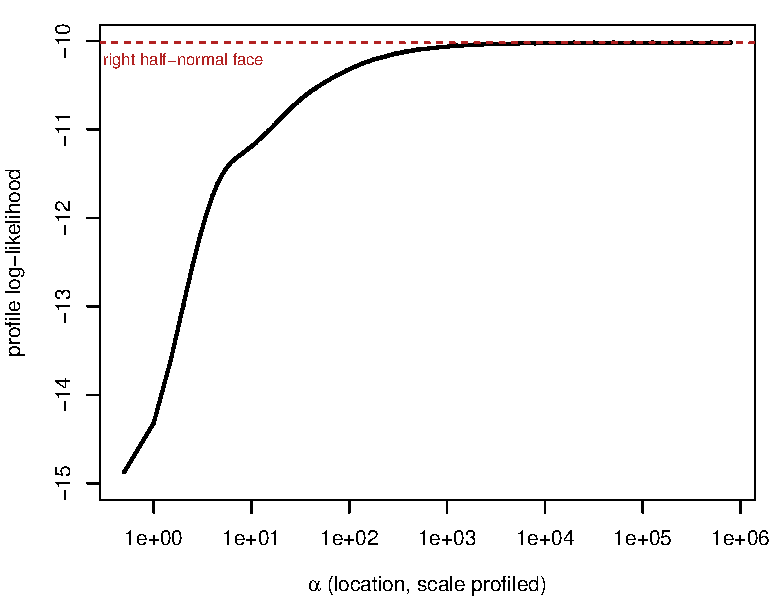
\includegraphics[width=0.62\textwidth]{failure-gallery/fig07-sn.pdf}
\caption{Profile log-likelihood over shape $\alpha$ (location and scale
profiled), against the right half-normal face; the dip-then-climb shape
explains why finite-magnitude divergence rules undercount escapes.}
\label{fig:sn}
\end{figure}

\section{Student-t: escape to the normal, and tie-collapse with free df}
\label{sec:std}

With mean, sd and $\nu$ all free, two distinct failures occur. (a) As
$\nu\to\infty$ the t tends to the normal; writing $K$ for the sample
kurtosis standardized at the normal MLE, the inward score of the profile
at the normal boundary is $\ell'_{\mathrm{profile}}(0^+)=n(K-3)/4$
(Johnson, Kotz and Balakrishnan 1995 \cite{jkb1995}), so $K\le3$ is
necessary for the normal to be the global supremum. (b) Independently of
(a), a tie of multiplicity $k$ makes the likelihood unbounded even with
$\nu$ \emph{held}, whenever $k>\nu(n-k)$ (scale collapses to zero at the
tied location); since the domain is $\nu>2$, this window is nonempty
exactly when $k>2(n-k)$, so a sufficiently large tie makes the
unrestricted (free-$\nu$) likelihood unbounded regardless of (a).

\begin{verbatim}
> mlstd(rnorm(200))
Error: The Student-t likelihood is maximised as nu -> Inf, i.e. by the
normal distribution. Use `mlnorm` to fit this model.

> x <- c(0, 0, 0, 0, 10)       # k = 4 at the tie, n - k = 1
> mlstd(x, nu = 3)             # 4 > 3*1: unbounded
Error: Likelihood is unbounded at a tie of excessive multiplicity
k > nu*(n-k) (free df: k > 2*(n-k)); no MLE.
> mlstd(x, nu = 5)             # 4 < 5*1: bounded
ok
\end{verbatim}
Figure~\ref{fig:std}(a) shows the profile over $\nu$ approaching the normal
logLik from below for the first sample; (b) shows the location-held scale
profile diverging at $\nu=3$ but not at $\nu=5$ for the second, confirming
the threshold exactly.

\begin{figure}[h]
\centering
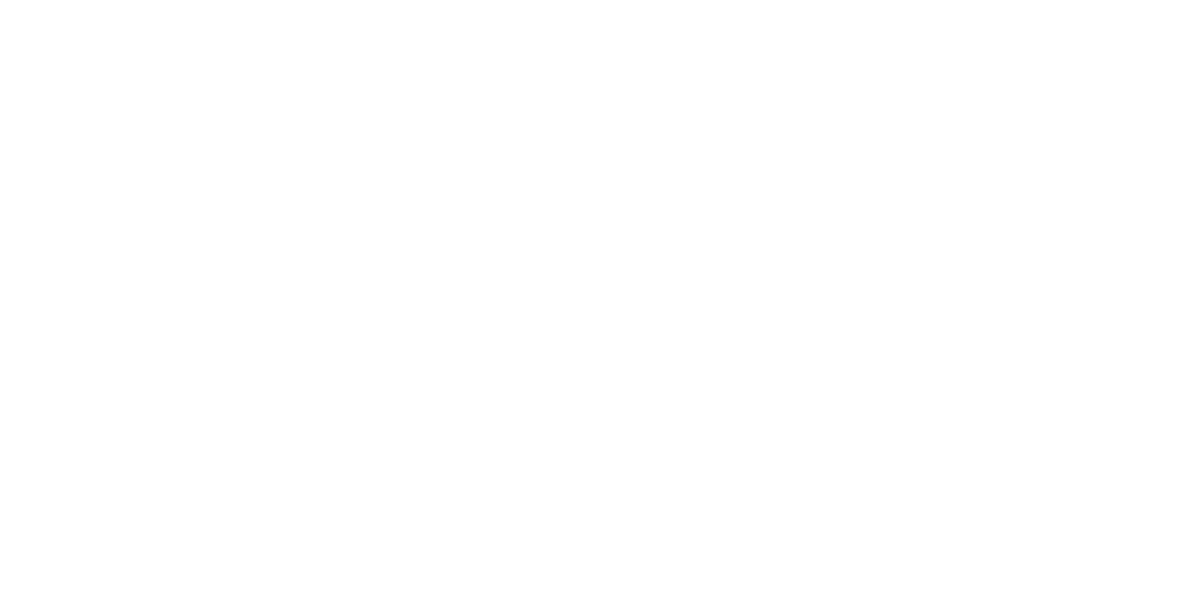
\includegraphics[width=\textwidth]{failure-gallery/fig08-std.pdf}
\caption{(a) Escape to the normal as $\nu\to\infty$. (b) Tie-collapse at a
held $\nu$ below and above the threshold $k/(n-k)=4$.}
\label{fig:std}
\end{figure}

\section{Free-threshold spikes: Pareto II, the generalized Pareto, and GED}
\label{sec:spikes}

Three unrelated families share the same mechanism: an unbounded
likelihood along a path that drives a single observation, or a single
endpoint, to a degenerate limit, fixed only by restricting the parameter
space (not by a numerical tolerance).

\emph{Pareto II, threshold free.} With $\mathrm{min}=m-\varepsilon$,
$\mathrm{scale}=\varepsilon$ ($m=\min x$, multiplicity $k$ there),
$L\propto\varepsilon^{\,\mathrm{shape}(n-k)-k}$, unbounded whenever
$\mathrm{shape}<k/(n-k)$; the package therefore requires a held threshold
(delegating to Lomax on $x-\mathrm{min}$;
\code{notes/evaluations/2026-10-29-threshold-report.md}).

\emph{Generalized Pareto, $\xi<-1$.} The upper endpoint
$\mathrm{mu}-\sigma/\xi$ is a density singularity for $\xi<-1$; sending it
down to $\max(x)$ from above drives the likelihood to $+\infty$. The
fitter restricts estimated $\xi\ge-1$ for exactly this reason
(\code{cppunivariate/.../distributions/gpd/README.md}).

\emph{GED, shape $\to0$.} With location at an observation and scale
profiled exactly, $\ell_p(\nu)/n=-\log q/\nu+\tfrac12\log\nu+O(1)\to\infty$
as $\nu\to0$ for every nonconstant sample (Tumlinson 2015
\cite{tumlinson2015}); the fitter restricts estimated $\nu\ge1$ (D6). A
\emph{held} $\nu$ away from zero, by contrast, is an ordinary well-posed
fit: the instability is specific to the joint limit, not to any fixed
sub-1 shape.

\begin{verbatim}
> x <- c(1, 2, 4, 7)
> mlpareto2(x, min = min(x) - 1e-4)   # logLik -6.586
> mlpareto2(x, min = min(x) - 1e-11)  # logLik  6.008, still rising

> y <- c(1, 2, 3, 7)   # max(y) = 7
> mlgpd(y, mu = 0, xi = -2, sigma = 2 * 8)        # endpoint 8: logLik -9.605
> mlgpd(y, mu = 0, xi = -2, sigma = 2 * 7.000001) # endpoint 7 + 1e-6: logLik -2.150

> mlged(x)             # restricted: nu = 2.095, logLik = -60.46
> mlged(x, nu = 0.3)    # held away from 0: ok, logLik = -72.63
\end{verbatim}

\begin{figure}[h]
\centering
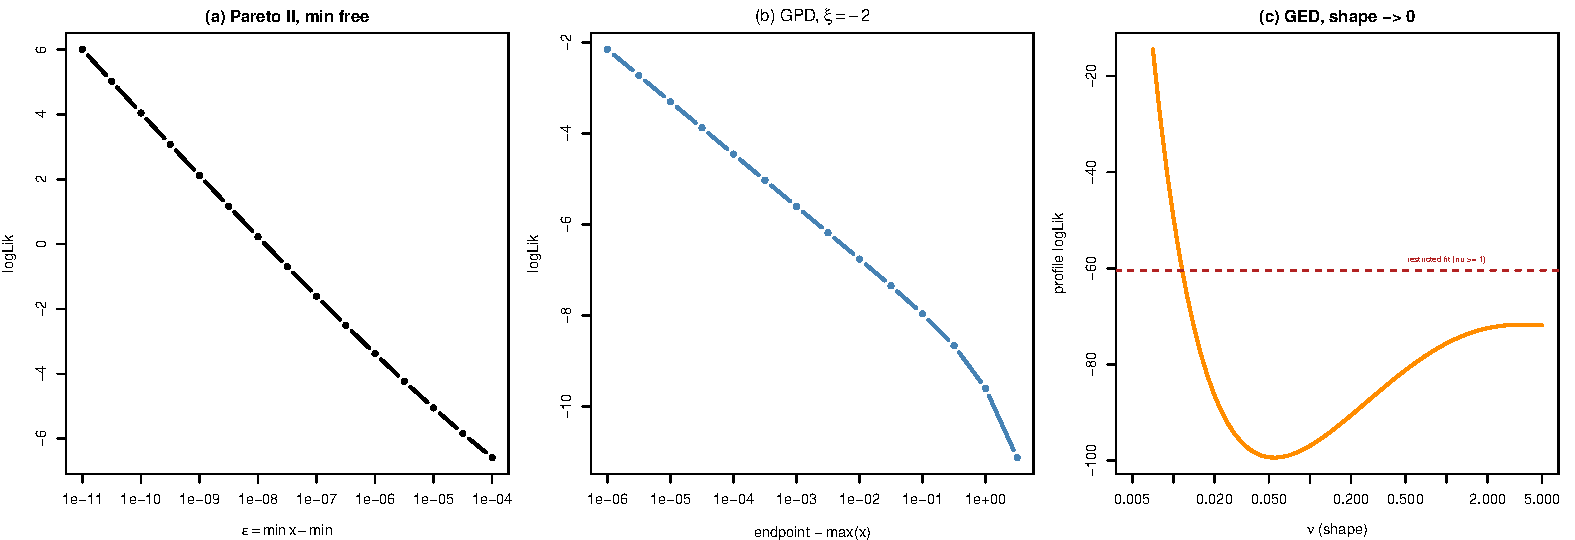
\includegraphics[width=\textwidth]{failure-gallery/fig09-spikes.pdf}
\caption{Three unbounded-likelihood mechanisms: (a) Pareto II with the
threshold free; (b) generalized Pareto with $\xi=-2$ held, endpoint sent to
$\max(x)$; (c) GED profile log-likelihood as shape $\to0$, against the
restricted fit at $\nu\ge1$.}
\label{fig:spikes}
\end{figure}

\section{Negative binomial, binomial and Lomax: escape to a smaller family}
\label{sec:exppois}

Two instances of the same shape: a family escapes, as one shape parameter
diverges with a product held fixed, to a strictly smaller-dimensional
family at its boundary.

\emph{Lomax $\to$ exponential.} $f(x)=\lambda\kappa(1+\lambda x)^{-(\kappa+1)}$
tends to $\mathrm{Exp}(\theta)$ as $\kappa\to\infty$, $\lambda\kappa\to\theta$.
With $q=\lambda\bar x$, $A(q)=n^{-1}\sum_i\log(1+qx_i/\bar x)$, the profile
gap is $\ell_p(\lambda)-\ell_E=n\{\log q-\log A(q)-A(q)\}$
(\code{notes/ml-behaviour.tex}, Theorem~1 there); the MLE exists iff this
gap is positive for some $q$, which fails whenever the sample coefficient
of variation is close enough to 1 (necessary below 1, not sufficient
above; del Castillo and Daoudi 2009 \cite{delcastillo2009}; Grimshaw 1993
\cite{grimshaw1993}).

\begin{verbatim}
> mllomax(c(1, 100))   # c = 0.980: kappa=0.4055 lambda=0.7722 logLik=-9.254
> mllomax(c(1, 10))    # c = 0.818
Error: The Lomax maximum likelihood estimator does not exist for data
whose likelihood is maximized on the exponential face. Use `mlexp`.
\end{verbatim}
The maximal gap for $(1,100)$ is $0.5901$ (Figure~\ref{fig:exppois}a,
matching the closed-form profile exactly); for $(1,10)$ the gap never
exceeds $0$.

\emph{Negative binomial / binomial $\to$ Poisson.} As
$\mathrm{size}\to\infty$ with the mean held, both discrete overdispersion
families tend to the Poisson (Johnson, Kemp and Kotz 2005
\cite{jkk2005}); detected at the fitter level as underdispersion
(population-form sample variance at or below the mean).

\begin{verbatim}
> x <- rpois(100, lambda = 5)
> mlnbinom(x)
Error: The maximum likelihood estimator does not exist for underdispersed
data, but converges to a Poisson. Use `mlpois` instead.
> mlpois(x)
lambda = 4.8700, logLik = -212.7134
\end{verbatim}
The size-profiled logLik increases monotonically and asymptotes to the
Poisson value (Figure~\ref{fig:exppois}b); \code{mlbinom} escapes the same
way when the free trial-size search is underdispersion-bound.

\begin{figure}[h]
\centering
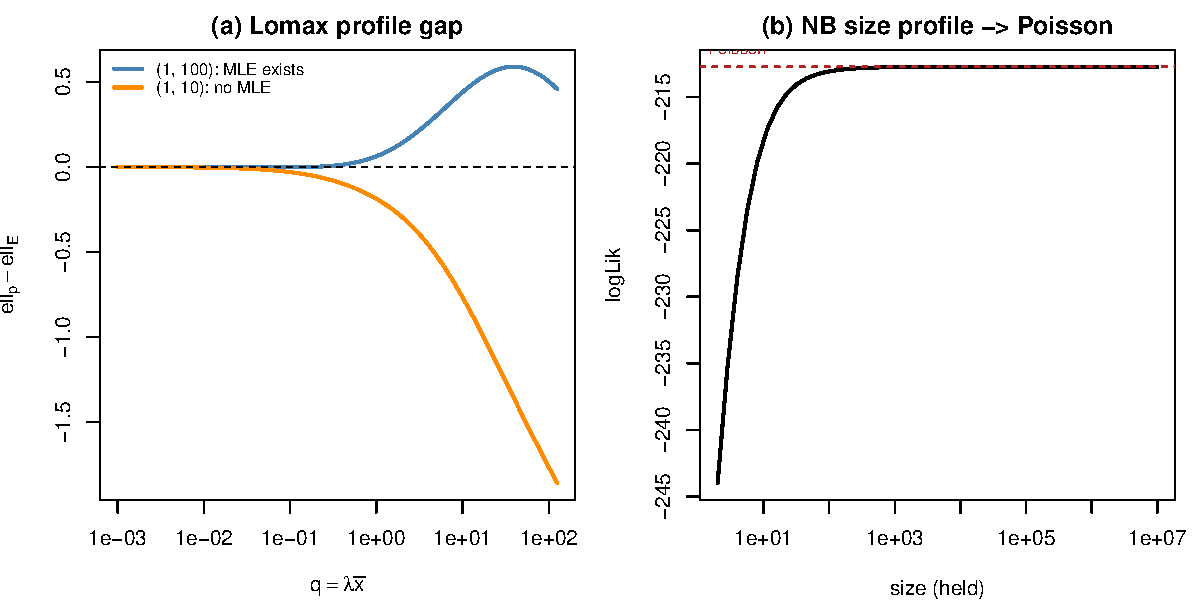
\includegraphics[width=\textwidth]{failure-gallery/fig10-exp-pois.pdf}
\caption{(a) Lomax profile gap $\ell_p(\lambda)-\ell_E$ for an existing and
a non-existing example. (b) Negative binomial size-profile approaching the
Poisson logLik.}
\label{fig:exppois}
\end{figure}

\begin{thebibliography}{99}

\bibitem{burridge1981} Burridge, J. (1981). A note on maximum likelihood
estimation for regression models using grouped data. \emph{Journal of the
Royal Statistical Society, Series B}, 43(1), 41--45.
\href{https://doi.org/10.1111/j.2517-6161.1981.tb01146.x}{doi:10.1111/j.2517-6161.1981.tb01146.x}.

\bibitem{kk2003} Kleiber, C. and Kotz, S. (2003). \emph{Statistical Size
Distributions in Economics and Actuarial Sciences}. Wiley.

\bibitem{joiner1971} Joiner, B. L. and Rosenblatt, J. R. (1971). Some
properties of the range in samples from Tukey's symmetric lambda
distributions. \emph{Journal of the American Statistical Association},
66(334), 394--399.
\href{https://doi.org/10.1080/01621459.1971.10482277}{doi:10.1080/01621459.1971.10482277}.

\bibitem{azzalini1985} Azzalini, A. (1985). A class of distributions which
includes the normal ones. \emph{Scandinavian Journal of Statistics}, 12,
171--178.

\bibitem{azzalinicapitanio1999} Azzalini, A. and Capitanio, A. (1999).
Statistical applications of the multivariate skew-normal distribution.
\emph{Journal of the Royal Statistical Society, Series B}, 61(3), 579--602.
\href{https://doi.org/10.1111/1467-9868.00194}{doi:10.1111/1467-9868.00194}.

\bibitem{pewsey2000} Pewsey, A. (2000). Problems of inference for
Azzalini's skew-normal distribution. \emph{Journal of Applied Statistics},
27(7), 859--870.
\href{https://doi.org/10.1080/02664760050120542}{doi:10.1080/02664760050120542}.

\bibitem{azzalinicapitanio2013} Azzalini, A. and Arellano-Valle, R. B.
(2013). Maximum penalized likelihood estimation for skew-normal and
skew-$t$ distributions. \emph{Journal of Statistical Planning and
Inference}, 143(2), 419--433.
\href{https://doi.org/10.1016/j.jspi.2012.06.022}{doi:10.1016/j.jspi.2012.06.022}.

\bibitem{jkb1995} Johnson, N. L., Kotz, S. and Balakrishnan, N. (1995).
\emph{Continuous Univariate Distributions, Volume 1} (2nd ed.), Chapter 13.
Wiley.

\bibitem{tumlinson2015} Tumlinson, S. E. (2015). On the non-existence of
maximum likelihood estimates for the extended exponential power
distribution and its generalizations. \emph{Statistics \& Probability
Letters}, 107, 111--114.
\href{https://doi.org/10.1016/j.spl.2015.08.009}{doi:10.1016/j.spl.2015.08.009}.

\bibitem{delcastillo2009} del Castillo, J. and Daoudi, J. (2009).
Estimation of the generalized Pareto distribution. \emph{Statistics \&
Probability Letters}, 79(5), 684--688.
\href{https://doi.org/10.1016/j.spl.2008.10.021}{doi:10.1016/j.spl.2008.10.021}.

\bibitem{grimshaw1993} Grimshaw, S. D. (1993). Computing maximum likelihood
estimates for the generalized Pareto distribution. \emph{Technometrics},
35(2), 185--191.
\href{https://doi.org/10.1080/00401706.1993.10485040}{doi:10.1080/00401706.1993.10485040}.

\bibitem{jkk2005} Johnson, N. L., Kemp, A. W. and Kotz, S. (2005).
\emph{Univariate Discrete Distributions} (3rd ed.). Wiley-Blackwell.

\end{thebibliography}

\end{document}
